
When quench propagates, the point at which the cable transforms from superconducting to normal state moves forward with time, as shown in Fig. \ref{fig:quench_front_propagation_illustration}. This point remains at critical temperature, $T_\text{c}$ for a given magnetic field strength. Its rate of position change in time is described as quench velocity. Depending on electro-magneto-thermal conditions at which quench occurs, quench velocity can remain constant or change in time. 

\begin{figure}[H]
\centering
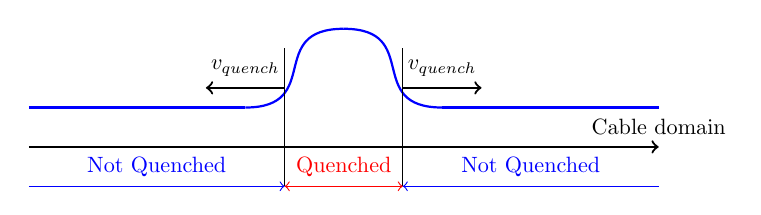
\begin{tikzpicture}[scale = 1]
\draw [thick, ->] (0.0,0.0) -- (8.0,0);

\draw [thick, blue] (0.0,0.5) -- (2.75,0.5);
\draw [thick, blue] (5.25,0.5) -- (8.0,0.5);

\draw [thick, blue] (2.75,0.5) .. controls +(0:1cm) and +(180:1cm) .. (4.0,1.5);
\draw [thick, blue] (4.0,1.5) .. controls +(0:1cm) and +(180:1cm) .. (5.25,0.5);

\draw [thin] (3.25,-0.5) -- (3.25,1.25);
\draw [thin] (4.75,-0.5) -- (4.75,1.25);

\draw [thick, ->] (4.75,0.75) -- (5.75,0.75);
\draw [thick, ->] (3.25,0.75) -- (2.25,0.75);

\draw [thin, red, <->] (3.25,-0.5) -- (4.75,-0.5);
\draw [thin, blue, ->] (0.0,-0.5) -- (3.25,-0.5);
\draw [thin, blue, <-] (4.75,-0.5) -- (8.0,-0.5);

\node[scale = 0.8] [color = red] at (4.0,-0.25) {Quenched};
\node[scale = 0.8] [color = blue] at (1.625,-0.25) {Not Quenched};
\node[scale = 0.8] [color = blue] at (6.375,-0.25) {Not Quenched};

\node[scale = 0.8] at (5.25,1.0) {$v_\text{quench}$};
\node[scale = 0.8] at (2.75,1.0) {$v_\text{quench}$};
\node[scale = 0.8] at (8.0,+0.25) {Cable domain};

\end{tikzpicture}
\caption{Quench velocity approach.}
\label{fig:quench_front_propagation_illustration}
\end{figure}

Quench velocity can be approximated with analytic formulas. They are usually a function of current density, material properties of the winding and temperature gradient around the quench front. The quench velocity in ITER applications is mainly estimated based on~\cite{MIT_phd_thesis}. For superconducting accelerator magnets, Wilson's formula is more applicable if cooling with helium is not considered \cite[p.~206]{wilson1987superconducting}, as described below
\begin{equation}
    v_\text{quench}=\frac{J}{\gamma C}\sqrt{\frac{\rho k}{T_\text{s}-T_\text{0}}},
    \label{eqn:Wilson_quench_velocity_formula}
\end{equation}
where $T_\text{s}$ -- critical temperature,
$T_\text{0}$ -- coolant temperature,
$\rho$ -- electrical resistivity averaged over the conductor volume,
$J$ -- current density averaged over the conductor volume,
$k$ -- thermal conductivity averaged over the conductor unit cell,
$C$ -- volumetric heat capacity averaged over the conductor unit cell,
$\gamma$ -- conductor density.